\documentclass{article}

% Language setting
% Replace `english' with e.g. `spanish' to change the document language
\usepackage[english]{babel}

% Set page size and margins
% Replace `letterpaper' with`a4paper' for UK/EU standard size
\usepackage[letterpaper,top=2cm,bottom=2cm,left=3cm,right=3cm,marginparwidth=1.75cm]{geometry}

% Useful packages
\usepackage{amsmath}
\usepackage{graphicx}
\usepackage[colorlinks=true, allcolors=blue]{hyperref}
\usepackage{tabularx}
\usepackage{fvextra}
\usepackage{ulem}


\usepackage{array,multirow,makecell}

\setcellgapes{1pt}
\makegapedcells
\newcolumntype{R}[1]{>{\raggedleft\arraybackslash }b{#1}}
\newcolumntype{L}[1]{>{\raggedright\arraybackslash }b{#1}}
\newcolumntype{C}[1]{>{\centering\arraybackslash }b{#1}}

\title{Rapport d'avancement}
\author{Vital FOCHEUX}
\date{du 18 juin au 26 juin}

\begin{document}

\maketitle

\section{Notes de la dernière réunion}

\begin{itemize}
    \item Savoir les performances en fonctions des ordres des différentes équations pour les filtres passe-bas et passe-haut
    \item Avoir un plan B si le compilateur n'est pas encore utilisable
    \item Utiliser d'autres valeurs pour les résultats des anti-windups
    \item Voir les résultats des anti-windups sans retenue (condition parfaite)
\end{itemize}

\section{Planning}

\begin{itemize}
    \item \sout{du 8 au 12 juin :} 
    \begin{itemize}
        \item \sout{Correction du modèle de drone $\rightarrow$ pour qu'il fonctionne avec une consigne plus cohérente (5 mètres) et qu'on observe des résultats différents entre avec/sans anti-windup}
        \item \sout{Séparation filtres/contrôleurs}
        \item \sout{Clarifier l'interface chips $\rightarrow$ montrer comment utiliser Filtre/Anti-windup en chips avec description bloc fonctionnel et documentation}
        \item \sout{Plan détaillé du rapport de stage}
    \end{itemize}
    \item du 15 au 19 juin :
    \begin{itemize}
        \item Rédaction du package contrôleur chips (diagramme bloc fonctionnel + chips) $\rightarrow$ tester (via BIP)
        \item Des plots et diagrammes (pour analyser les résultats)
        \item Mise en commun avec Julien (travaux futurs)
    \end{itemize}
    \item du 22 au 26 juin :
    \begin{itemize}
        \item Rédaction du rapport de stage
        \item Lien formel travaux Vital / Motif control
    \end{itemize}
\end{itemize}

\section{Depuis la dernière fois}

\subsection{Filtre}

Actuellement, les filtres passe-bas et passe-haut sont du premier ordre discrétisé par Backward Euler :
$$H(s) = \frac{1}{\tau s + 1}$$

Ces filtres permet de réduire les bruits présent sur les mesures. Cependant, les essais ont montré que le filtrage reste limité.
(cf. figures\ref{fig:lowpass_order1}, \ref{fig:lowpass_fft_order1}, \ref{fig:lowpass_psd_order1}, \ref{fig:highpass_order1}, \ref{fig:highpass_fft_order1}, \ref{fig:highpass_psd_order1}) \\
Pour amélioirer le filtrage, on pouvais augmenter la constante de temps $\tau$ mais cela entraîne :
\begin{itemize}
    \item davantage de retard
    \item une perte de réactivité
\end{itemize}

Le filtre Butterworth pour le passe-bas et passe-haut d'ordre 2 est une solution pour améliorer le filtrage.
Pourquoi le Butterworth ? Car il possède une propriété intéressante : il a une réponse en fréquence la plus plate possible dans la bande passante. Cela signifie qu'il n'y a pas de ondulations dans la bande passante, ce qui est souhaitable pour de nombreuses applications.

Je ne choisi pas un filtre d'ordre supérieur car :
\begin{itemize}
    \item le retard de phase augmente
    \item la compléxité augmente
    \item le réglage devient plus délicat
\end{itemize}

Le Butterworth d'ordre 2 constitue donc un compromis raisonnable entre :
\begin{itemize}
    \item efficacité du filtrage
    \item simplicité d'implémentation
    \item coût de calcul
\end{itemize}

\begin{figure}
    \centering
    
\includegraphics[width=\textwidth]{low_pass_order1.png}
    \caption{Résultat du filtre passe-bas d'ordre 1 sur des fréquences avec du bruit}
    \label{fig:lowpass_order1}
\end{figure}

\begin{figure}
    \centering
    
\includegraphics[width=\textwidth]{low_pass_fft_order1.png}
    \caption{Spectre fréquentiel du signal avant et après filtre passe-bas d'ordre 1}
    \label{fig:lowpass_fft_order1}
\end{figure}

\begin{figure}
    \centering
    
\includegraphics[width=\textwidth]{low_pass_psd_order1.png}
    \caption{Densité spectrale de puissance avant et après filtre passe-bas d'ordre 1}
    \label{fig:lowpass_psd_order1}
\end{figure}

\begin{figure}
    \centering
    
\includegraphics[width=\textwidth]{low_pass_order2.png}
    \caption{Résultat du filtre passe-bas d'ordre 2 sur des fréquences avec du bruit}
    \label{fig:lowpass_order2}
\end{figure}

\begin{figure}
    \centering
    
\includegraphics[width=\textwidth]{low_pass_fft_order2.png}
    \caption{Spectre fréquentiel du signal avant et après filtre passe-bas d'ordre 2}
    \label{fig:lowpass_fft_order2}
\end{figure}

\begin{figure}
    \centering
    
\includegraphics[width=\textwidth]{low_pass_psd_order2.png}
    \caption{Densité spectrale de puissance avant et après filtre passe-bas d'ordre 2}
    \label{fig:lowpass_psd_order2}
\end{figure}

\begin{figure}
    \centering
    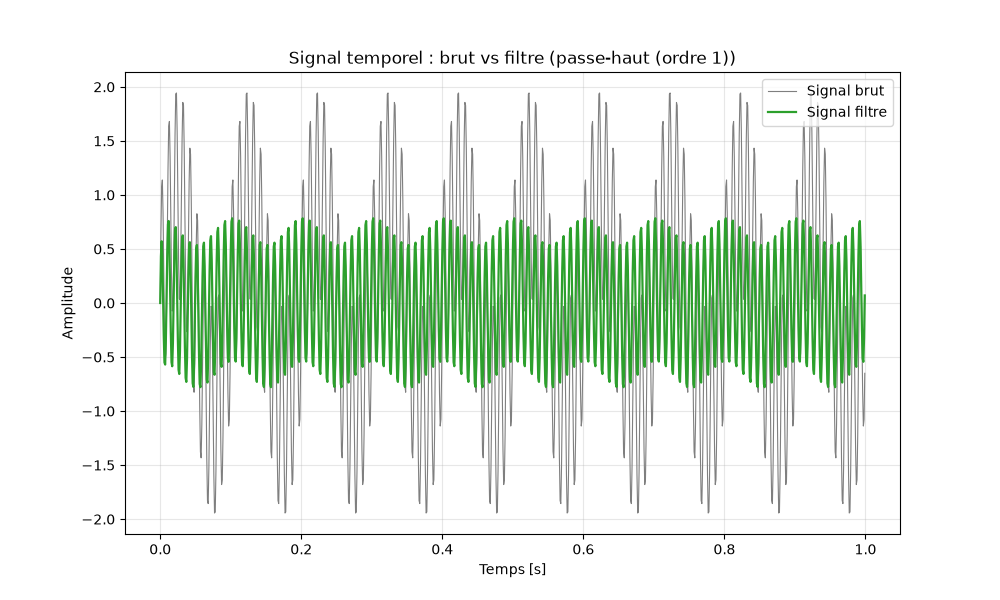
\includegraphics[width=\textwidth]{high_pass_order1.png}
    \caption{Résultat du filtre passe-haut d'ordre 1 sur des fréquences avec du bruit}
    \label{fig:highpass_order1}
\end{figure}

\begin{figure}
    \centering
    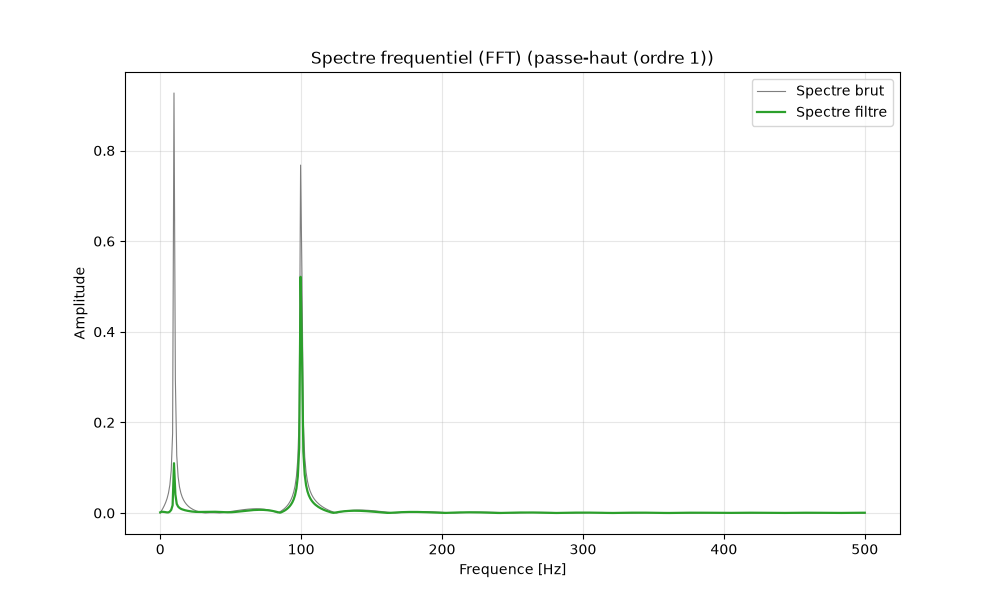
\includegraphics[width=\textwidth]{high_pass_fft_order1.png}
    \caption{Spectre fréquentiel du signal avant et après filtre passe-haut d'ordre 1}
    \label{fig:highpass_fft_order1}
\end{figure}

\begin{figure}
    \centering
    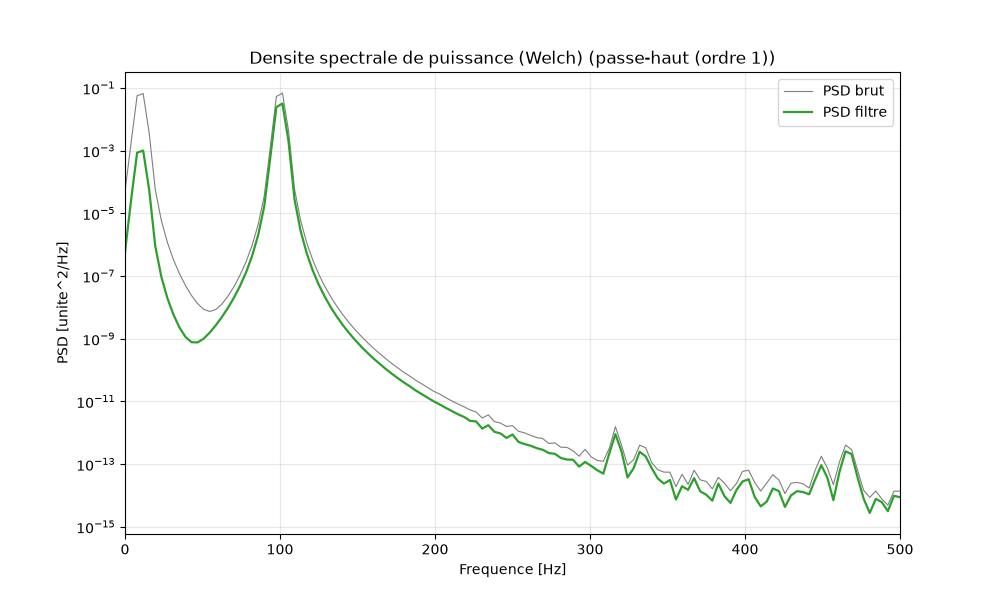
\includegraphics[width=\textwidth]{high_pass_psd_order1.png}
    \caption{Densité spectrale de puissance avant et après filtre passe-haut d'ordre 1}
    \label{fig:highpass_psd_order1}
\end{figure}

\begin{figure}
    \centering
    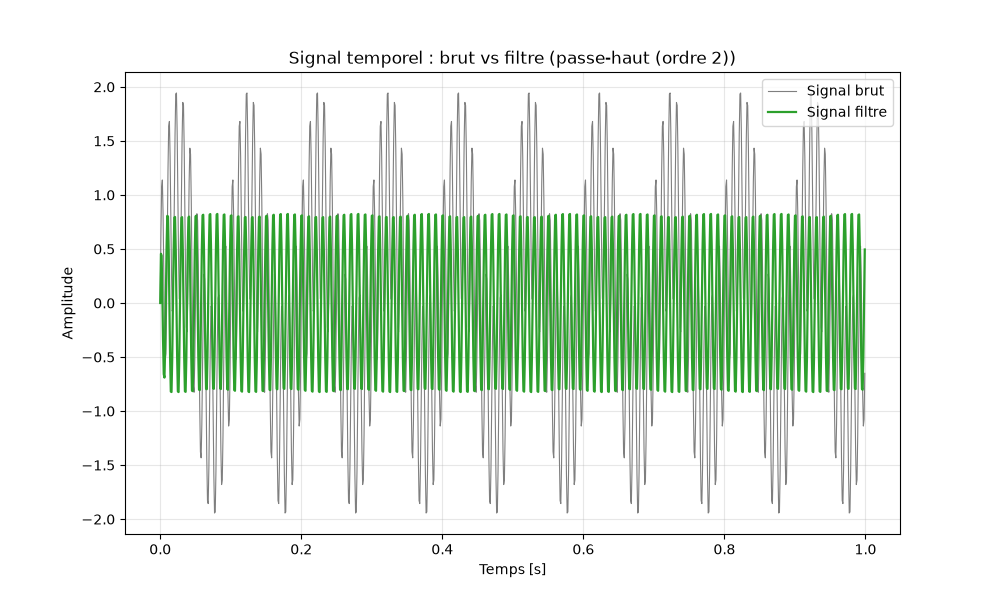
\includegraphics[width=\textwidth]{high_pass_order2.png}
    \caption{Résultat du filtre passe-haut d'ordre 2 sur des fréquences avec du bruit}
    \label{fig:highpass_order2}
\end{figure}

\begin{figure}
    \centering
    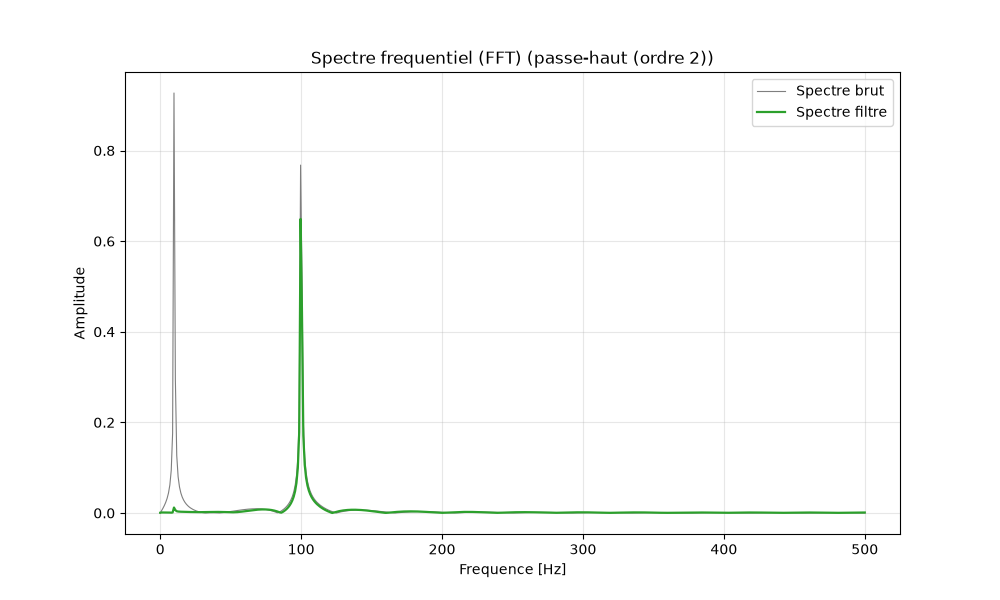
\includegraphics[width=\textwidth]{high_pass_fft_order2.png}
    \caption{Spectre fréquentiel du signal avant et après filtre passe-haut d'ordre 2}
    \label{fig:highpass_fft_order2}
\end{figure}

\begin{figure}
    \centering
    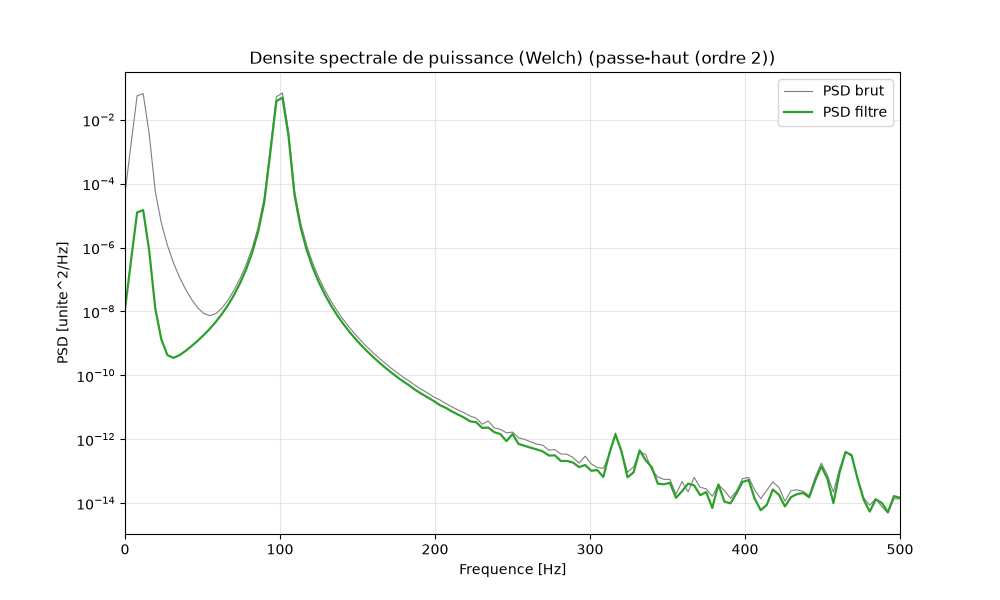
\includegraphics[width=\textwidth]{high_pass_psd_order2.png}
    \caption{Densité spectrale de puissance avant et après filtre passe-haut d'ordre 2}
    \label{fig:highpass_psd_order2}
\end{figure}

\subsection{Anti-windup}

\begin{figure}
    \centering
    
\includegraphics[width=\textwidth]{anti_windup_altitude.png}
    \caption{Altitude du drone avec différents anti-windups avec la retenue}
    \label{fig:antiwindup_alt_retenue}
\end{figure}

\begin{figure}
    \centering
    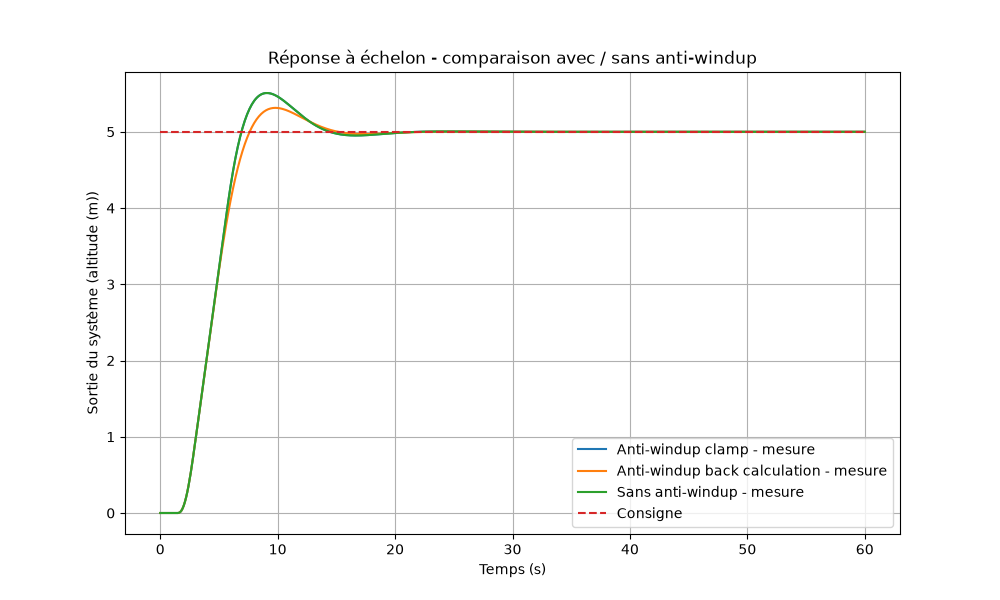
\includegraphics[width=\textwidth]{anti_windup_altitude_sans_retenue.png}
    \caption{Altitude du drone avec différents anti-windups sans la retenue}
    \label{fig:antiwindup_alt_sans_retenue}
\end{figure}

\begin{figure}
    \centering
    
\includegraphics[width=\textwidth]{anti_windup_integral.png}
    \caption{Intégrale des différents anti-windups avec la retenue}
    \label{fig:antiwindup_integral_retenue}
\end{figure}

\begin{figure}
    \centering
    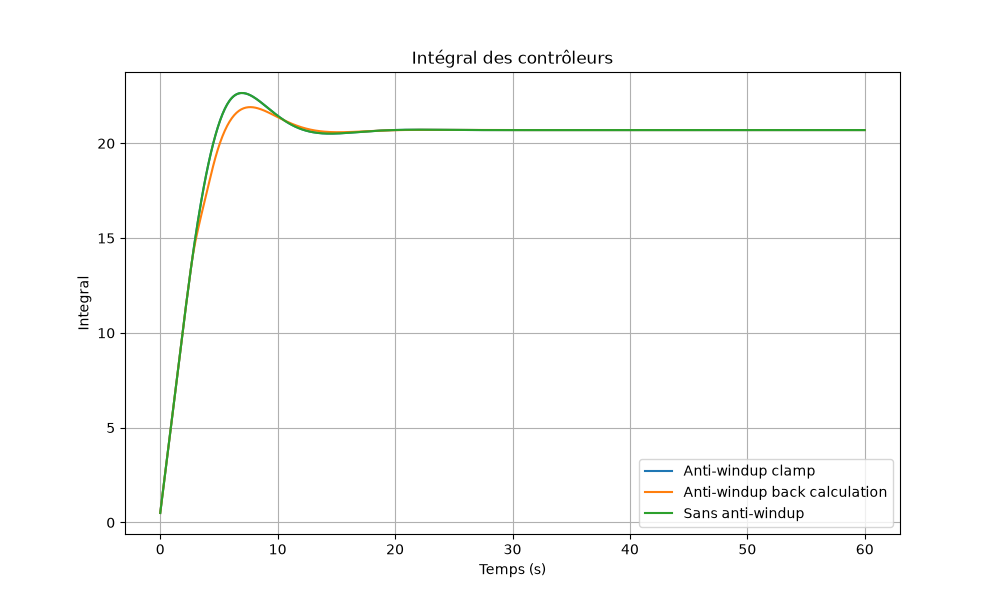
\includegraphics[width=\textwidth]{anti_windup_integral_sans_retenue.png}
    \caption{Intégrale des différents anti-windups sans la retenue}
    \label{fig:antiwindup_integral_sans_retenue}
\end{figure}

\begin{figure}
    \centering
    
\includegraphics[width=\textwidth]{anti_windup_blade.png}
    \caption{Vitesse de rotation des hélices avec différents anti-windups avec retenue}
    \label{fig:antiwindup_blade}
\end{figure}

\begin{figure}
    \centering
    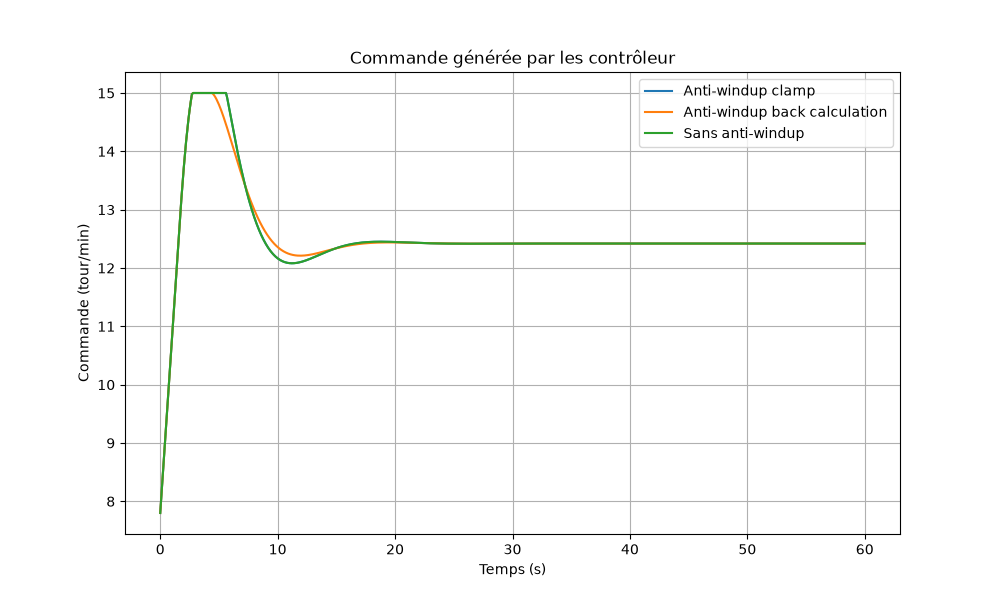
\includegraphics[width=\textwidth]{anti_windup_blade_sans_retenue.png}
    \caption{Vitesse de rotation des hélices avec différents anti-windups sans retenue}
    \label{fig:antiwindup_blade_sans_retenue}
\end{figure}

Les résultats avec la retenue de 10 secondes

\begin{tabular}{|c|c|c|}
    \hline & Altitute max (m) & Dépassement maximal (\%) \\
    \hline Sans anti-windup & 12 & 140 \\
    \hline Anti-windup clamp & 7.32 & 46 \\
    \hline Anti-windup back-calculation & 5.31 & 6.2 \\
    \hline 
\end{tabular}

\begin{tabular}{|c|c|c|}
    \hline & Temps de stabilisation ($\pm 5\%$) (s) & Intégrale maximale \\
    \hline Sans anti-windup & 32.2 & 60.86 \\
    \hline Anti-windup clamp & 21.6 & 30 \\
    \hline Anti-windup back-calculation & 18.9 & 21.9 \\
    \hline
\end{tabular}



\begin{tabular}{|C{3.5cm}|C{3.5cm}|C{3.5cm}|C{3.5cm}|}
    \hline & Commande maximale (tour/min) & Commande minimale local (tour/min) & Commande moyenne (tour/min) \\
    \hline Sans anti-windup & 15 & 7.13 & 12.78 \\
    \hline Anti-windup clamp & 15 & 10.82 & 12.86 \\
    \hline Anti-windup back-calculation & 15 & 12.21 & 12.88 \\
    \hline
\end{tabular}

Les résultats sans la retenue de 10 secondes

\begin{tabular}{|c|c|c|}
    \hline & Altitute max (m) & Dépassement maximal (\%) \\
    \hline Sans anti-windup & 5.5 & 10 \\
    \hline Anti-windup clamp & 5.5 & 10 \\
    \hline Anti-windup back-calculation & 5.31 & 6.2 \\
    \hline 
\end{tabular}

\begin{tabular}{|c|c|c|}
    \hline & Temps de stabilisation ($\pm 5\%$) (s) & Intégrale maximale \\
    \hline Sans anti-windup & 11.8 & 22.6 \\
    \hline Anti-windup clamp & 11.8 & 22.6 \\
    \hline Anti-windup back-calculation & 11.3 & 21.9 \\
    \hline
\end{tabular}



\begin{tabular}{|C{3.5cm}|C{3.5cm}|C{3.5cm}|C{3.5cm}|}
    \hline & Commande maximale (tour/min) & Commande minimale local (tour/min) & Commande moyenne (tour/min) \\
    \hline Sans anti-windup & 15 & 12.08 & 12.54 \\
    \hline Anti-windup clamp & 15 & 12.08 & 12.54 \\
    \hline Anti-windup back-calculation & 15 & 12.21 & 12.54 \\
    \hline
\end{tabular}

\subsection{Mise en place de toolchain}

Le compilateur est maintenant fonctionnel. J'ai pu mettre en place la toolchain permettant de parser un programme CHIPS, le sérialiser en XMI, analyser que le XMI généré est conforme au métamodèle, puis générer le code XMI pour BIP pour enfin compiler vers du code BIP.
La toolchain a mis du temps pour être fonctionnelle car il y avait des petits problèmes un peu de partout donc le temps de débugger, les résoudre\dots il fallu du temps.
Mais maintenant qu'elle est en place je vais pouvoir écrire des programme CHIPS et tester les contrôleurs écrit en C++.

\end{document}